
\chapter{Using Buffers, Windows, and Frames}
\begin{figure}[!ht]
  \centering
  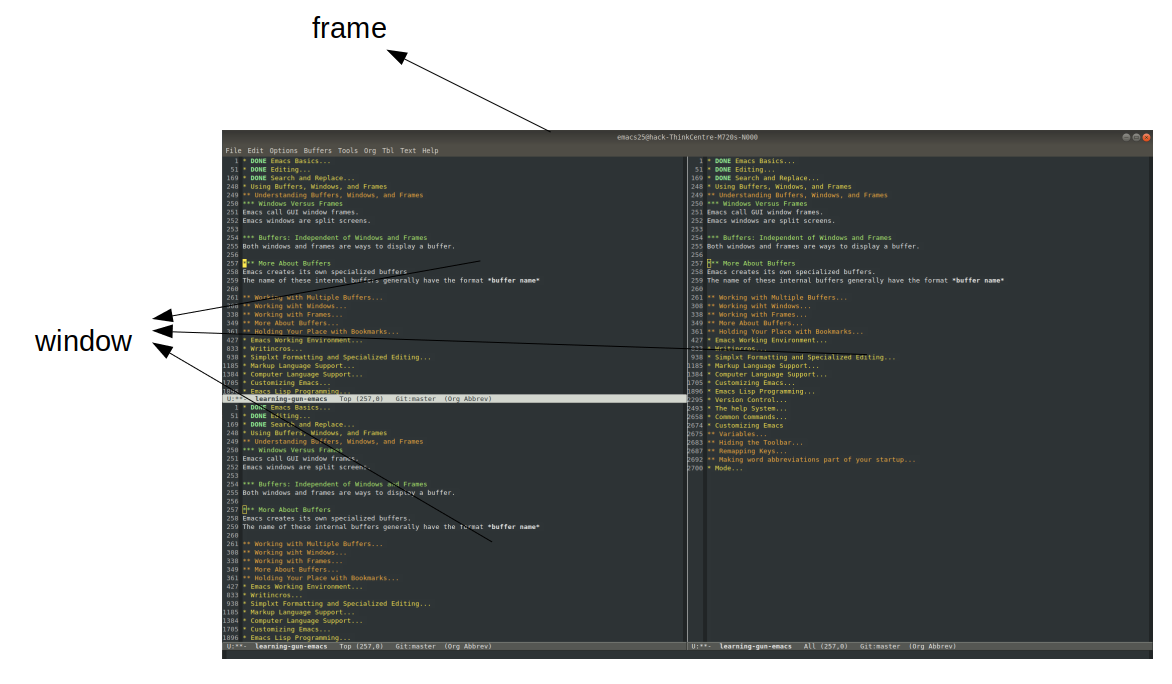
\includegraphics[width=\textwidth]{frame-windows.png}
  \caption{Frame and Window}
  \label{fig:frame-and-window}
\end{figure}

Emacs call GUI window frames.
Emacs windows are split screens.
Both windows and frames are ways to display a buffer.
Emacs creates its own specialized buffers.
The name of these internal buffers generally have the format \keyword{buffer name}.

\section{Buffers}
\begin{description}
\item[C-x b] Switch to the most recently opened buffer.
\item[C-x C-b] List all buffers.
\item[C-x k] Kill the current buffer.
\item[C-x s] Save all buffers.
\item[C-x C-q] toggle read only mode                    
\item[C-x 4 r] open a file as read-only in a new window 
\item[C-x 5 r] open a file as read-only in a new frame  
\end{description}

\section{Windows}
\begin{description}
\item[C-x o] Switch to other window.
\item[C-x 0] Delete the current window.
\item[C-x 1] Delete other windows.
\item[C-x 2] Split window vertically.
\item[C-x 3] Split window right.
\item[C-x \^{}] Enlarge window.
\item[C-x \}] Enlarge window horizontally.
\item[C-x \{] Shrink window horizontally.
\item[C-x -] Shrink window if larger than buffer.
\item[C-x +] Balance window.
\end{description}

\section{Frames}
\begin{description}
\item[C-x 5 o] other-frame        
\item[C-x 5 0] delete-frame       
\item[C-x 5 1] delete-other-frame 
\item[C-x 5 2] make-frame-command 
\end{description}


